% Journal of Emerging Investigators (JEI) Submission
% Heterogeneous GNN for Celiac Gut-Brain Axis

\documentclass[12pt]{article}

\usepackage[utf8]{inputenc}
\usepackage[margin=1in]{geometry}
\usepackage{graphicx}
\usepackage{amsmath}
\usepackage{amssymb}
\usepackage{booktabs}
\usepackage{multirow}
\usepackage{hyperref}
\usepackage{natbib}
\usepackage{lineno}
\usepackage{xcolor}
\usepackage{subcaption}

% JEI requires line numbers
\linenumbers

\title{Modeling the Celiac Gut-Brain Axis with Heterogeneous Graph Neural Networks}

\author{
    [Author Name]\\
    [School Name]\\
    [City, State]\\
    \texttt{[email]}
}

\date{}

\begin{document}

\maketitle

% =============================================================================
\begin{abstract}
Celiac disease (CeD) affects approximately 1\% of the global population and is associated with neurological manifestations including cerebellar ataxia, peripheral neuropathy, and cognitive dysfunction in 10--22\% of patients. However, the biological mechanisms connecting intestinal inflammation to brain pathology remain poorly understood. We present a computational approach using heterogeneous graph neural networks (HeteroGNNs) to model the celiac gut-brain axis. Our knowledge graph integrates 225 nodes across four biological entity types---gut microbes (n=14), microbial metabolites (n=12), immune/metabolic genes (n=113), and neurological phenotypes (n=86)---connected by 229 curated relationships. Using link prediction, our model achieves an AUROC of $0.905 \pm 0.050$ on gene-phenotype associations across five random seeds. Ablation studies demonstrate that removing metabolite nodes decreases performance by 4.8\%, while removing all intermediate nodes (microbes and metabolites) decreases performance by 6.0\%, indicating that multi-hop reasoning through metabolic intermediates contributes meaningfully to prediction accuracy. This work demonstrates how graph-based machine learning can generate testable hypotheses for complex multi-system diseases affecting the gut-brain axis.
\end{abstract}

\textbf{Keywords:} celiac disease, gut-brain axis, graph neural networks, knowledge graph, microbiome, neurological manifestations

% =============================================================================
\section{Introduction}

Celiac disease (CeD) is an autoimmune disorder triggered by dietary gluten in genetically susceptible individuals, primarily those carrying HLA-DQ2 or HLA-DQ8 haplotypes \citep{lebwohl2018celiac}. While traditionally characterized as an intestinal disease causing villous atrophy and malabsorption, CeD is increasingly recognized as a systemic condition with diverse extra-intestinal manifestations \citep{caio2019celiac}.

Neurological complications represent a significant but underappreciated burden of celiac disease. Population-based studies report neurological symptoms in 10--22\% of celiac patients, including:
\begin{itemize}
    \item \textbf{Gluten ataxia}: Cerebellar dysfunction with gait instability and dysarthria
    \item \textbf{Peripheral neuropathy}: Sensory and motor nerve damage
    \item \textbf{Cognitive impairment}: Memory difficulties and ``brain fog''
    \item \textbf{Psychiatric symptoms}: Depression and anxiety at 2--3$\times$ baseline rates
\end{itemize}

The mechanisms connecting intestinal inflammation to neurological symptoms remain incompletely understood. Three major hypotheses have been proposed:
\begin{enumerate}
    \item \textbf{Immune-mediated pathway}: Cross-reactive antibodies, particularly anti-transglutaminase 6 (TG6) antibodies, may target brain tissue \citep{hadjivassiliou2008autoantibodies}
    \item \textbf{Microbiome-mediated pathway}: Altered gut bacteria produce neuroactive metabolites (serotonin precursors, short-chain fatty acids) that influence brain function via the vagus nerve and systemic circulation \citep{dinan2017gutbrain}
    \item \textbf{Nutrient deficiency pathway}: Malabsorption of B vitamins, iron, and other micronutrients affects neurological function
\end{enumerate}

Understanding these complex, multi-step biological connections requires integrating diverse data types across multiple scales. Knowledge graphs provide a natural framework for representing heterogeneous biomedical relationships, and graph neural networks (GNNs) can learn from these complex structures to predict novel associations \citep{zhang2022graph}.

In this study, we construct a curated knowledge graph representing the celiac gut-brain axis and apply heterogeneous GNNs to predict gene-phenotype associations. Our approach:
\begin{enumerate}
    \item Demonstrates that GNN-based link prediction can achieve high accuracy on this biomedical task
    \item Quantifies the contribution of different biological intermediates (microbes, metabolites) through systematic ablation studies
    \item Identifies candidate pathways connecting intestinal dysbiosis to neurological manifestations
\end{enumerate}

% =============================================================================
\section{Methods}

\subsection{Knowledge Graph Construction}

We constructed a heterogeneous knowledge graph integrating four biological entity types and eleven relationship types relevant to celiac disease and gut-brain communication (Figure~\ref{fig:kg_schema}).

\begin{figure}[h]
\centering
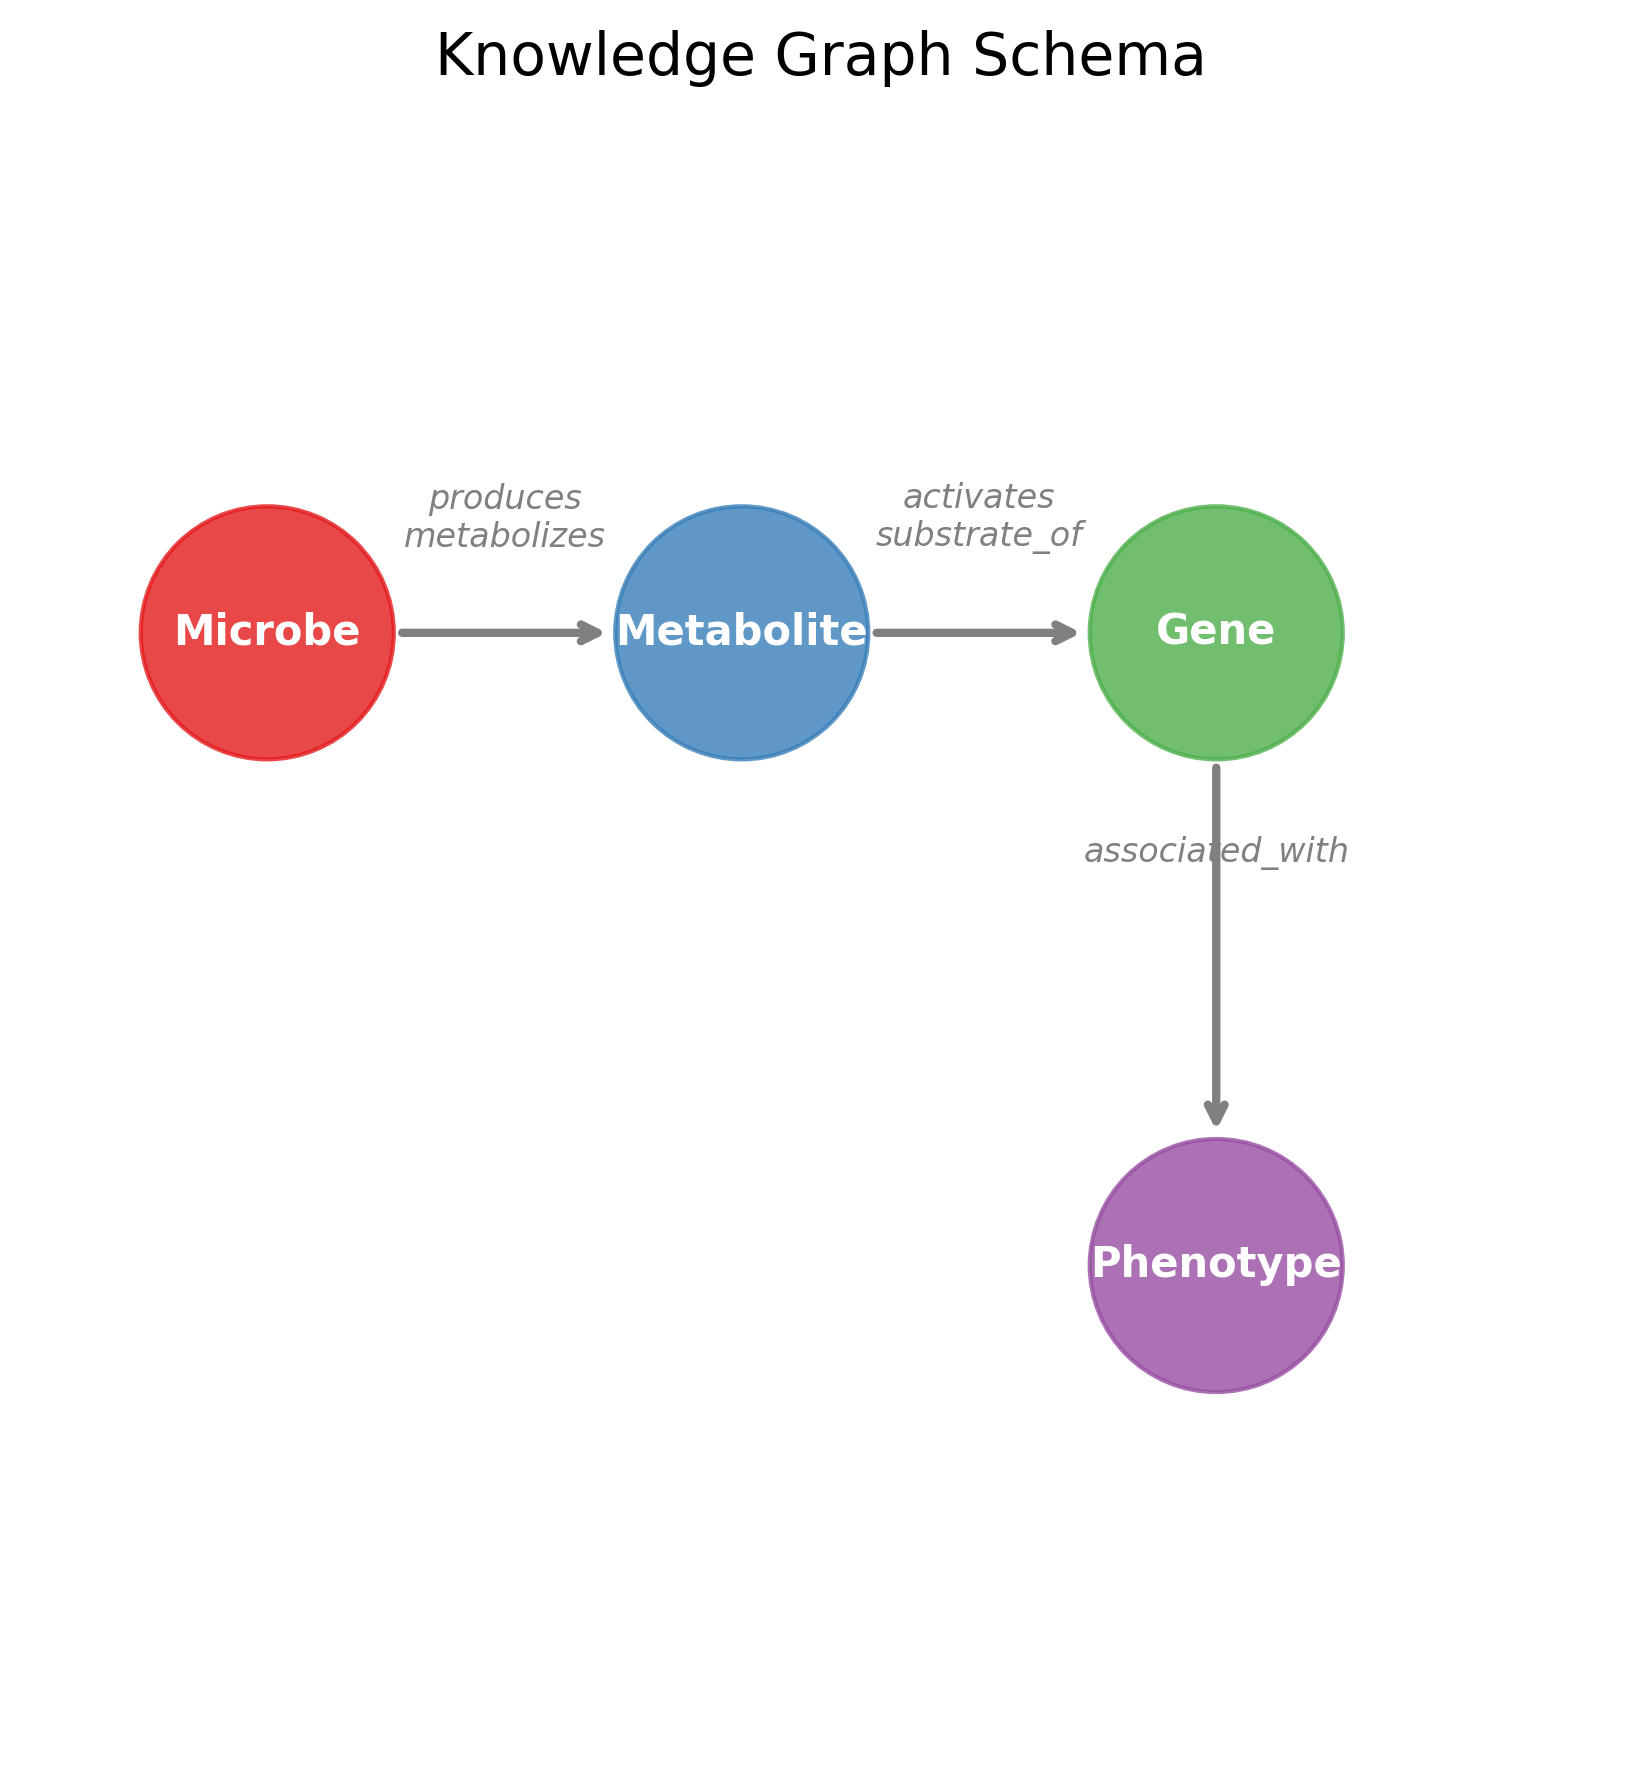
\includegraphics[width=0.85\textwidth]{../../figures/kg_schema.png}
\caption{Knowledge graph schema showing the four node types (Microbe, Metabolite, Gene, Phenotype) and their relationships. Edges represent biological interactions such as metabolite production by microbes, gene activation by metabolites, and gene-phenotype associations from the Monarch Initiative.}
\label{fig:kg_schema}
\end{figure}

\subsubsection{Node Types}

\begin{itemize}
    \item \textbf{Microbe nodes} (n=14): Gut bacteria with documented alterations in celiac disease, selected from meta-analyses of 16S rRNA sequencing studies \citep{arcila2022microbiome}. Examples include \textit{Prevotella}, \textit{Bifidobacterium}, and \textit{Lactobacillus} species.

    \item \textbf{Metabolite nodes} (n=12): Neuroactive compounds produced or modulated by gut microbiota, including short-chain fatty acids (butyrate, propionate, acetate), tryptophan metabolites (serotonin, kynurenine), and neurotransmitter precursors (GABA, dopamine precursors).

    \item \textbf{Gene nodes} (n=113): Human genes involved in immune function (HLA-DQ, interleukins, TNF), neurotransmitter metabolism (TPH1/2, SLC6A4, MAOA), and gut-brain signaling (FFAR2/3, GPR41).

    \item \textbf{Phenotype nodes} (n=86): Human Phenotype Ontology (HPO) terms representing neurological and gastrointestinal symptoms associated with celiac disease, including ataxia, neuropathy, cognitive impairment, and enteropathy.
\end{itemize}

\subsubsection{Edge Types}

Relationships were curated from published literature and existing databases:

\begin{itemize}
    \item \textbf{Microbe $\rightarrow$ Metabolite} (n=21 edges): Production, metabolism, and modulation relationships from metabolomic studies
    \item \textbf{Metabolite $\rightarrow$ Gene} (n=19 edges): Activation, substrate, and transport relationships from pathway databases
    \item \textbf{Gene $\rightarrow$ Phenotype} (n=187 edges): Disease associations from the Monarch Initiative knowledge base, which aggregates data from OMIM, ClinVar, and model organism databases
\end{itemize}

The final knowledge graph contains \textbf{225 nodes} and \textbf{229 edges} (Table~\ref{tab:kg_stats}).

\begin{table}[h]
\centering
\caption{Knowledge Graph Statistics}
\label{tab:kg_stats}
\begin{tabular}{lcc}
\toprule
\textbf{Entity Type} & \textbf{Node Count} & \textbf{Outgoing Edges} \\
\midrule
Microbe & 14 & 21 \\
Metabolite & 12 & 19 \\
Gene & 113 & 187 \\
Phenotype & 86 & -- \\
\midrule
\textbf{Total} & \textbf{225} & \textbf{227} \\
\bottomrule
\end{tabular}
\end{table}

\subsection{Heterogeneous Graph Neural Network Architecture}

We implemented a heterogeneous GNN using PyTorch Geometric \citep{fey2019pyg}. The architecture processes the multi-relational graph structure while respecting node and edge type heterogeneity.

\subsubsection{Node Embeddings}

Each node is initialized with a learnable embedding vector $\mathbf{h}_i^{(0)} \in \mathbb{R}^{d}$, where $d=64$ is the embedding dimension. Separate embedding tables are maintained for each node type.

\subsubsection{Message Passing Layers}

We employ two layers of heterogeneous graph convolutions based on GraphSAGE \citep{hamilton2017graphsage}. For each edge type $(s, r, t)$ connecting source type $s$ to target type $t$ via relation $r$, the update rule is:

\begin{equation}
    \mathbf{h}_j^{(\ell+1)} = \sigma\left(\mathbf{W}_r^{(\ell)} \cdot \text{AGGREGATE}\left(\{\mathbf{h}_i^{(\ell)} : i \in \mathcal{N}_r(j)\}\right)\right)
\end{equation}

where $\mathcal{N}_r(j)$ denotes neighbors of node $j$ via relation $r$, $\mathbf{W}_r^{(\ell)}$ are relation-specific learnable weights, and $\sigma$ is the ReLU activation function. After aggregation across all edge types, dropout ($p=0.3$) is applied for regularization.

\subsubsection{Link Prediction Decoder}

For the gene-phenotype link prediction task, we use a bilinear decoder:
\begin{equation}
    s_{ij} = \mathbf{h}_i^{(L)} \cdot \mathbf{W}_{decode} \cdot \mathbf{h}_j^{(L)}
\end{equation}

where $\mathbf{h}_i^{(L)}$ and $\mathbf{h}_j^{(L)}$ are the final-layer embeddings of gene $i$ and phenotype $j$, and $\mathbf{W}_{decode}$ is a learnable weight matrix.

\subsubsection{Training Objective}

The model is trained to minimize binary cross-entropy loss over positive (observed) and negative (sampled) edges:
\begin{equation}
    \mathcal{L} = -\frac{1}{|E^+| + |E^-|}\left[\sum_{(i,j) \in E^+} \log \sigma(s_{ij}) + \sum_{(i,j) \in E^-} \log(1 - \sigma(s_{ij}))\right]
\end{equation}

where $E^+$ are positive edges and $E^-$ are randomly sampled negative edges at a 1:1 ratio.

\subsection{Experimental Setup}

\subsubsection{Data Splitting}
Gene-phenotype edges were randomly split into training (70\%), validation (15\%), and test (15\%) sets. Negative edges were sampled uniformly from non-existing gene-phenotype pairs.

\subsubsection{Training Protocol}
Models were trained using the Adam optimizer with learning rate 0.01 for up to 100 epochs. Early stopping with patience of 20 epochs was applied based on validation AUROC. All experiments were repeated with 5 random seeds (0, 1, 2, 42, 123) to assess stability.

\subsubsection{Evaluation Metrics}
We report Area Under the ROC Curve (AUROC) and Area Under the Precision-Recall Curve (AUPRC) as primary metrics, following standard practice for link prediction tasks.

\subsubsection{Ablation Studies}
To quantify the contribution of different node types, we performed ablation experiments removing:
\begin{enumerate}
    \item Microbe nodes (and all connected edges)
    \item Metabolite nodes (and all connected edges)
    \item Both microbe and metabolite nodes (direct gene-phenotype only)
\end{enumerate}

% =============================================================================
\section{Results}

\subsection{Knowledge Graph Statistics}

Figure~\ref{fig:kg_stats} illustrates the distribution of nodes and edges in our curated knowledge graph. Gene nodes dominate numerically (50\% of nodes), reflecting the comprehensive annotation of gene-phenotype associations in the Monarch Initiative database.

\begin{figure}[h]
\centering
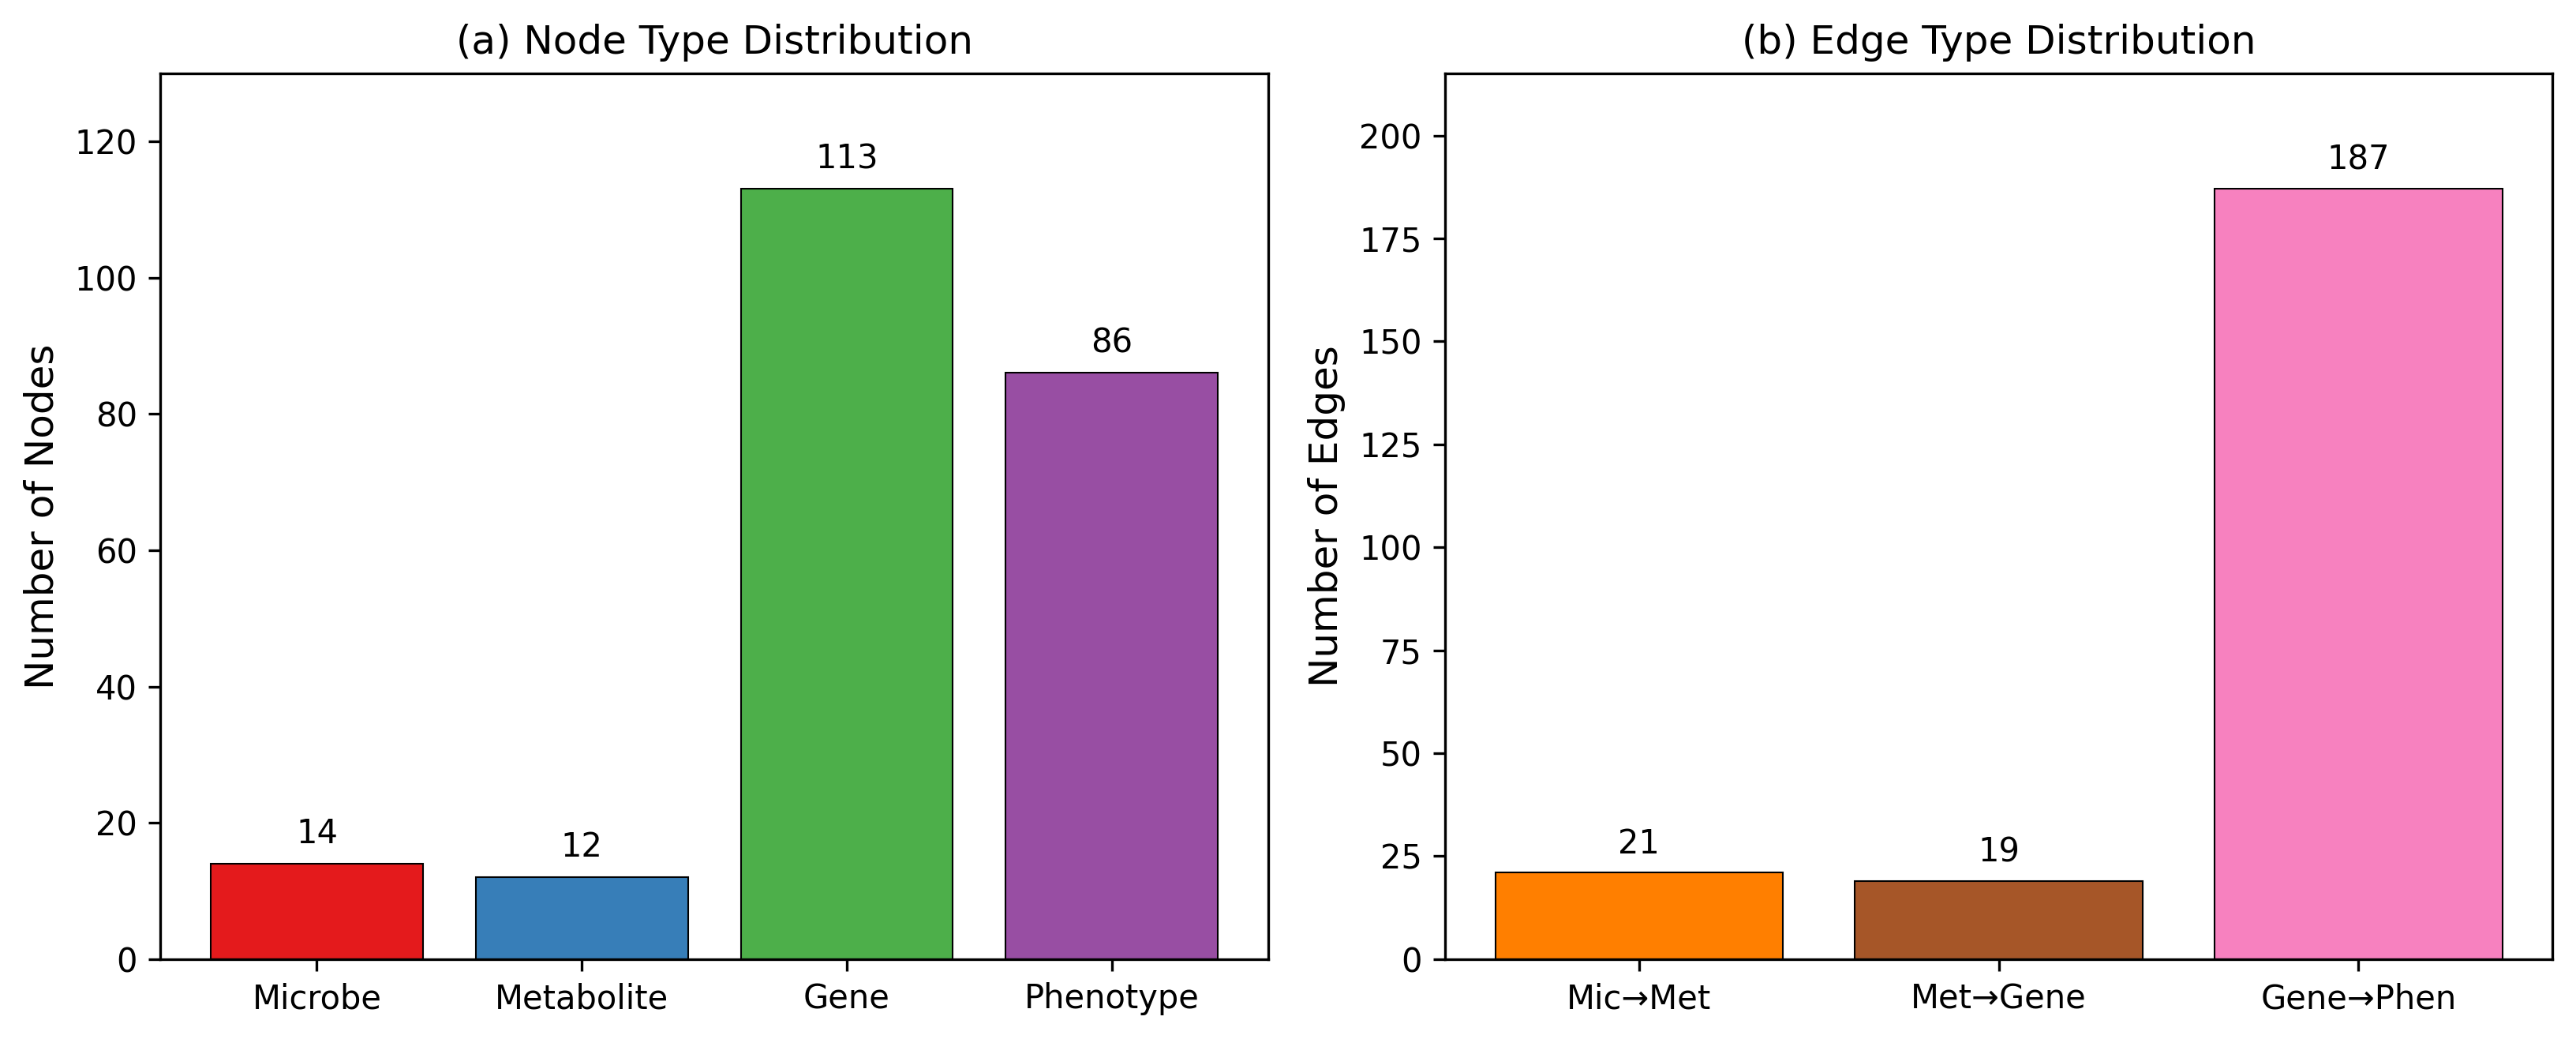
\includegraphics[width=\textwidth]{../../figures/kg_statistics.png}
\caption{Knowledge graph composition. \textbf{(a)} Node type distribution showing genes as the largest category. \textbf{(b)} Edge type distribution showing gene-phenotype associations as the dominant edge type, with microbe-metabolite and metabolite-gene edges providing multi-hop connectivity.}
\label{fig:kg_stats}
\end{figure}

\subsection{Link Prediction Performance}

The heterogeneous GNN achieved strong performance on the gene-phenotype link prediction task. Across five random seeds, the model achieved:

\begin{itemize}
    \item \textbf{Test AUROC}: $0.905 \pm 0.050$
    \item \textbf{Test AUPRC}: $0.896 \pm 0.038$
    \item \textbf{Validation AUROC}: $0.904 \pm 0.045$
\end{itemize}

Table~\ref{tab:results} summarizes the main results.

\begin{table}[h]
\centering
\caption{Link Prediction Performance (Mean $\pm$ Std over 5 Seeds)}
\label{tab:results}
\begin{tabular}{lcc}
\toprule
\textbf{Metric} & \textbf{Validation} & \textbf{Test} \\
\midrule
AUROC & $0.904 \pm 0.045$ & $0.905 \pm 0.050$ \\
AUPRC & $0.913 \pm 0.046$ & $0.896 \pm 0.038$ \\
\bottomrule
\end{tabular}
\end{table}

Training converged rapidly, with early stopping triggered at a mean of $22.2 \pm 16.1$ epochs. Figure~\ref{fig:training} shows representative training curves.

\begin{figure}[h]
\centering
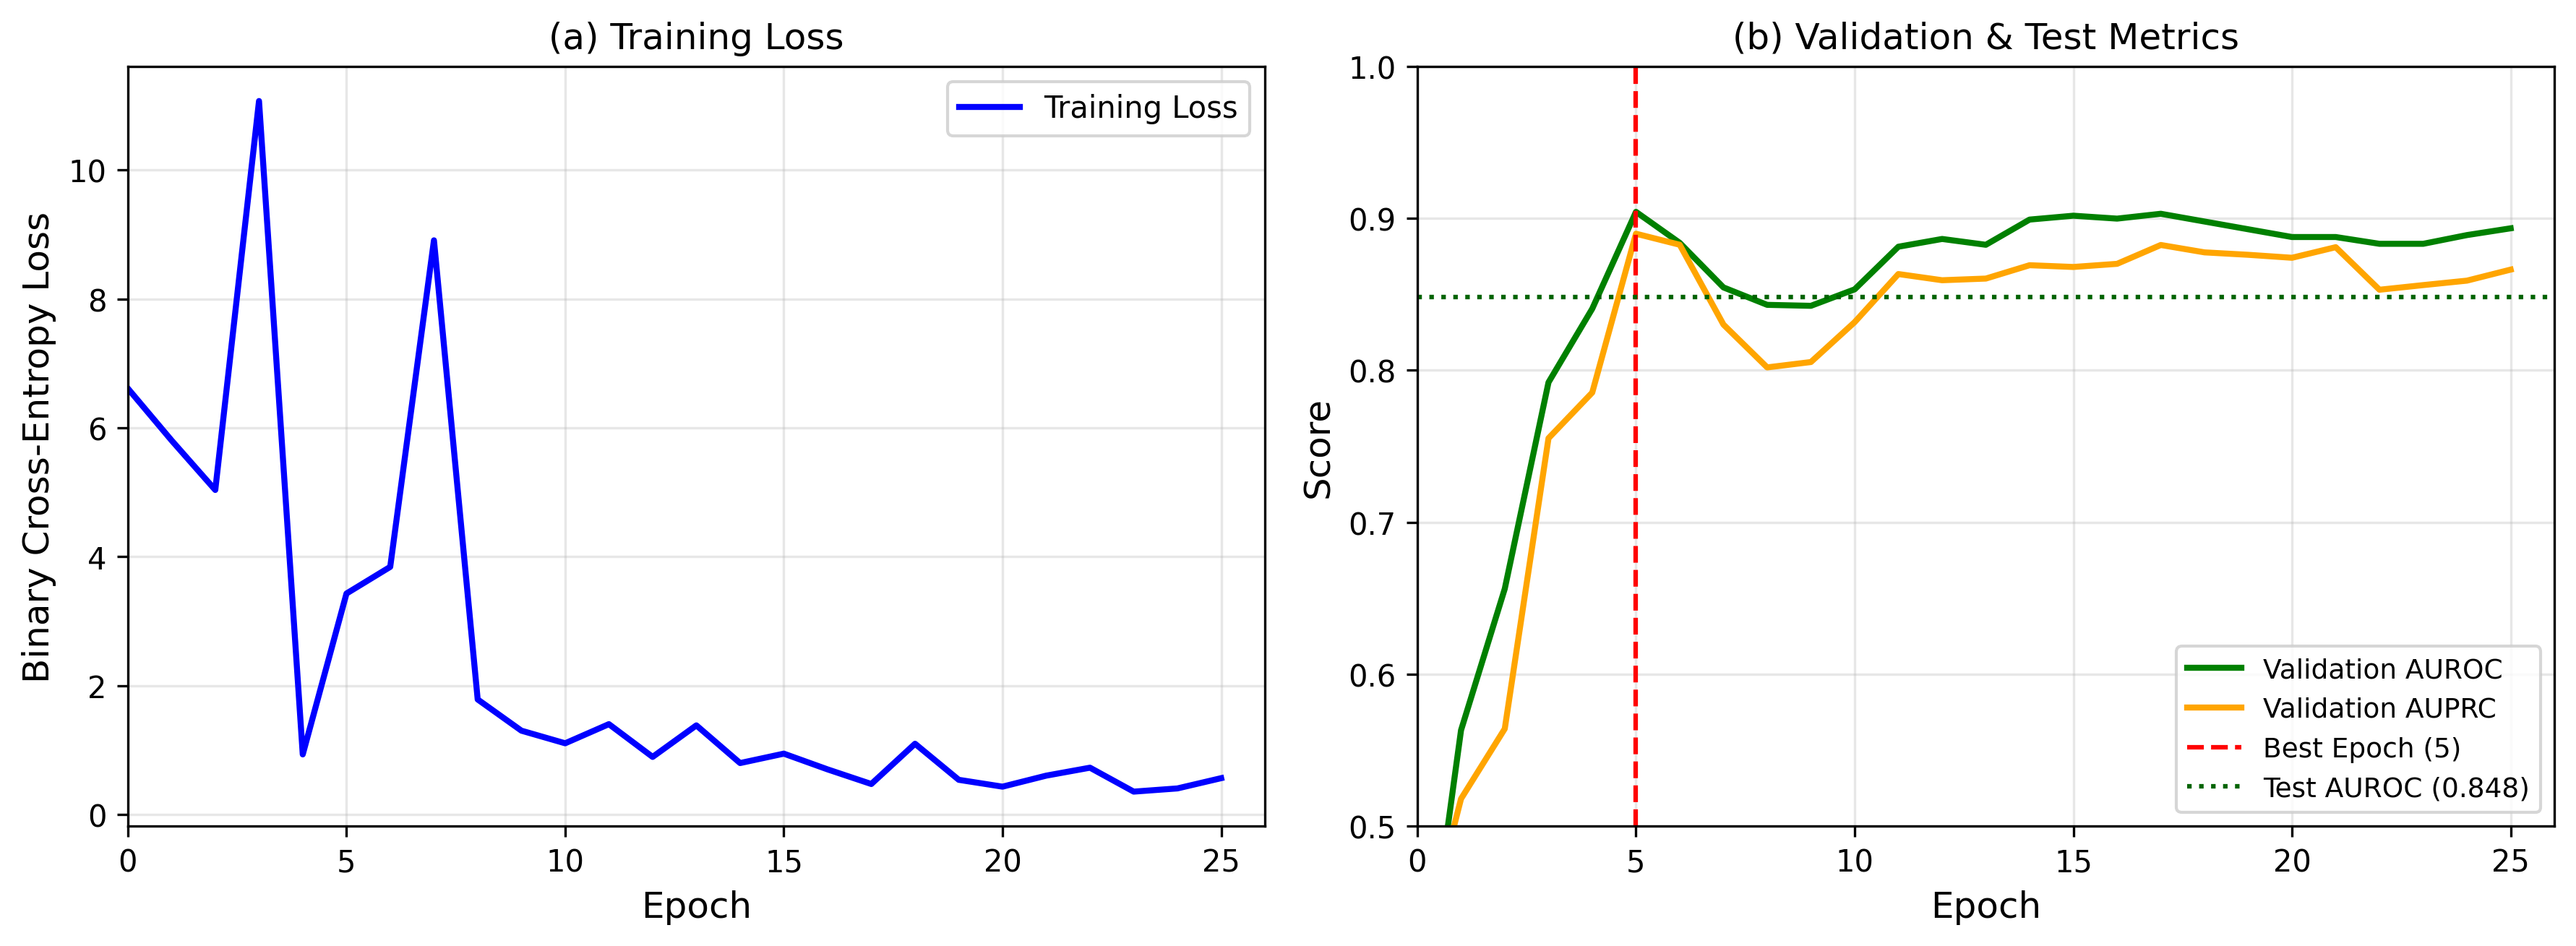
\includegraphics[width=\textwidth]{../../figures/training_curves.png}
\caption{Training dynamics. \textbf{(a)} Training loss decreases rapidly, indicating effective optimization. \textbf{(b)} Validation AUROC and AUPRC converge to high values, with the best model selected by early stopping. Test AUROC (dashed line) closely matches validation performance.}
\label{fig:training}
\end{figure}

\subsection{Ablation Studies: Contribution of Biological Intermediates}

To understand which components of the knowledge graph contribute to prediction performance, we conducted systematic ablation experiments (Table~\ref{tab:ablation}, Figure~\ref{fig:ablation}).

\begin{table}[h]
\centering
\caption{Ablation Study Results (Mean $\pm$ Std over 5 Seeds)}
\label{tab:ablation}
\begin{tabular}{lccc}
\toprule
\textbf{Configuration} & \textbf{AUROC} & \textbf{AUPRC} & \textbf{$\Delta$ AUROC} \\
\midrule
Full graph (baseline) & $0.905 \pm 0.050$ & $0.896 \pm 0.038$ & -- \\
Remove microbe nodes & $0.868 \pm 0.096$ & $0.852 \pm 0.082$ & $-4.1\%$ \\
Remove metabolite nodes & $0.861 \pm 0.034$ & $0.858 \pm 0.043$ & $-4.8\%$ \\
Direct gene-phenotype only & $0.850 \pm 0.061$ & $0.841 \pm 0.096$ & $-6.0\%$ \\
\bottomrule
\end{tabular}
\end{table}

\begin{figure}[h]
\centering
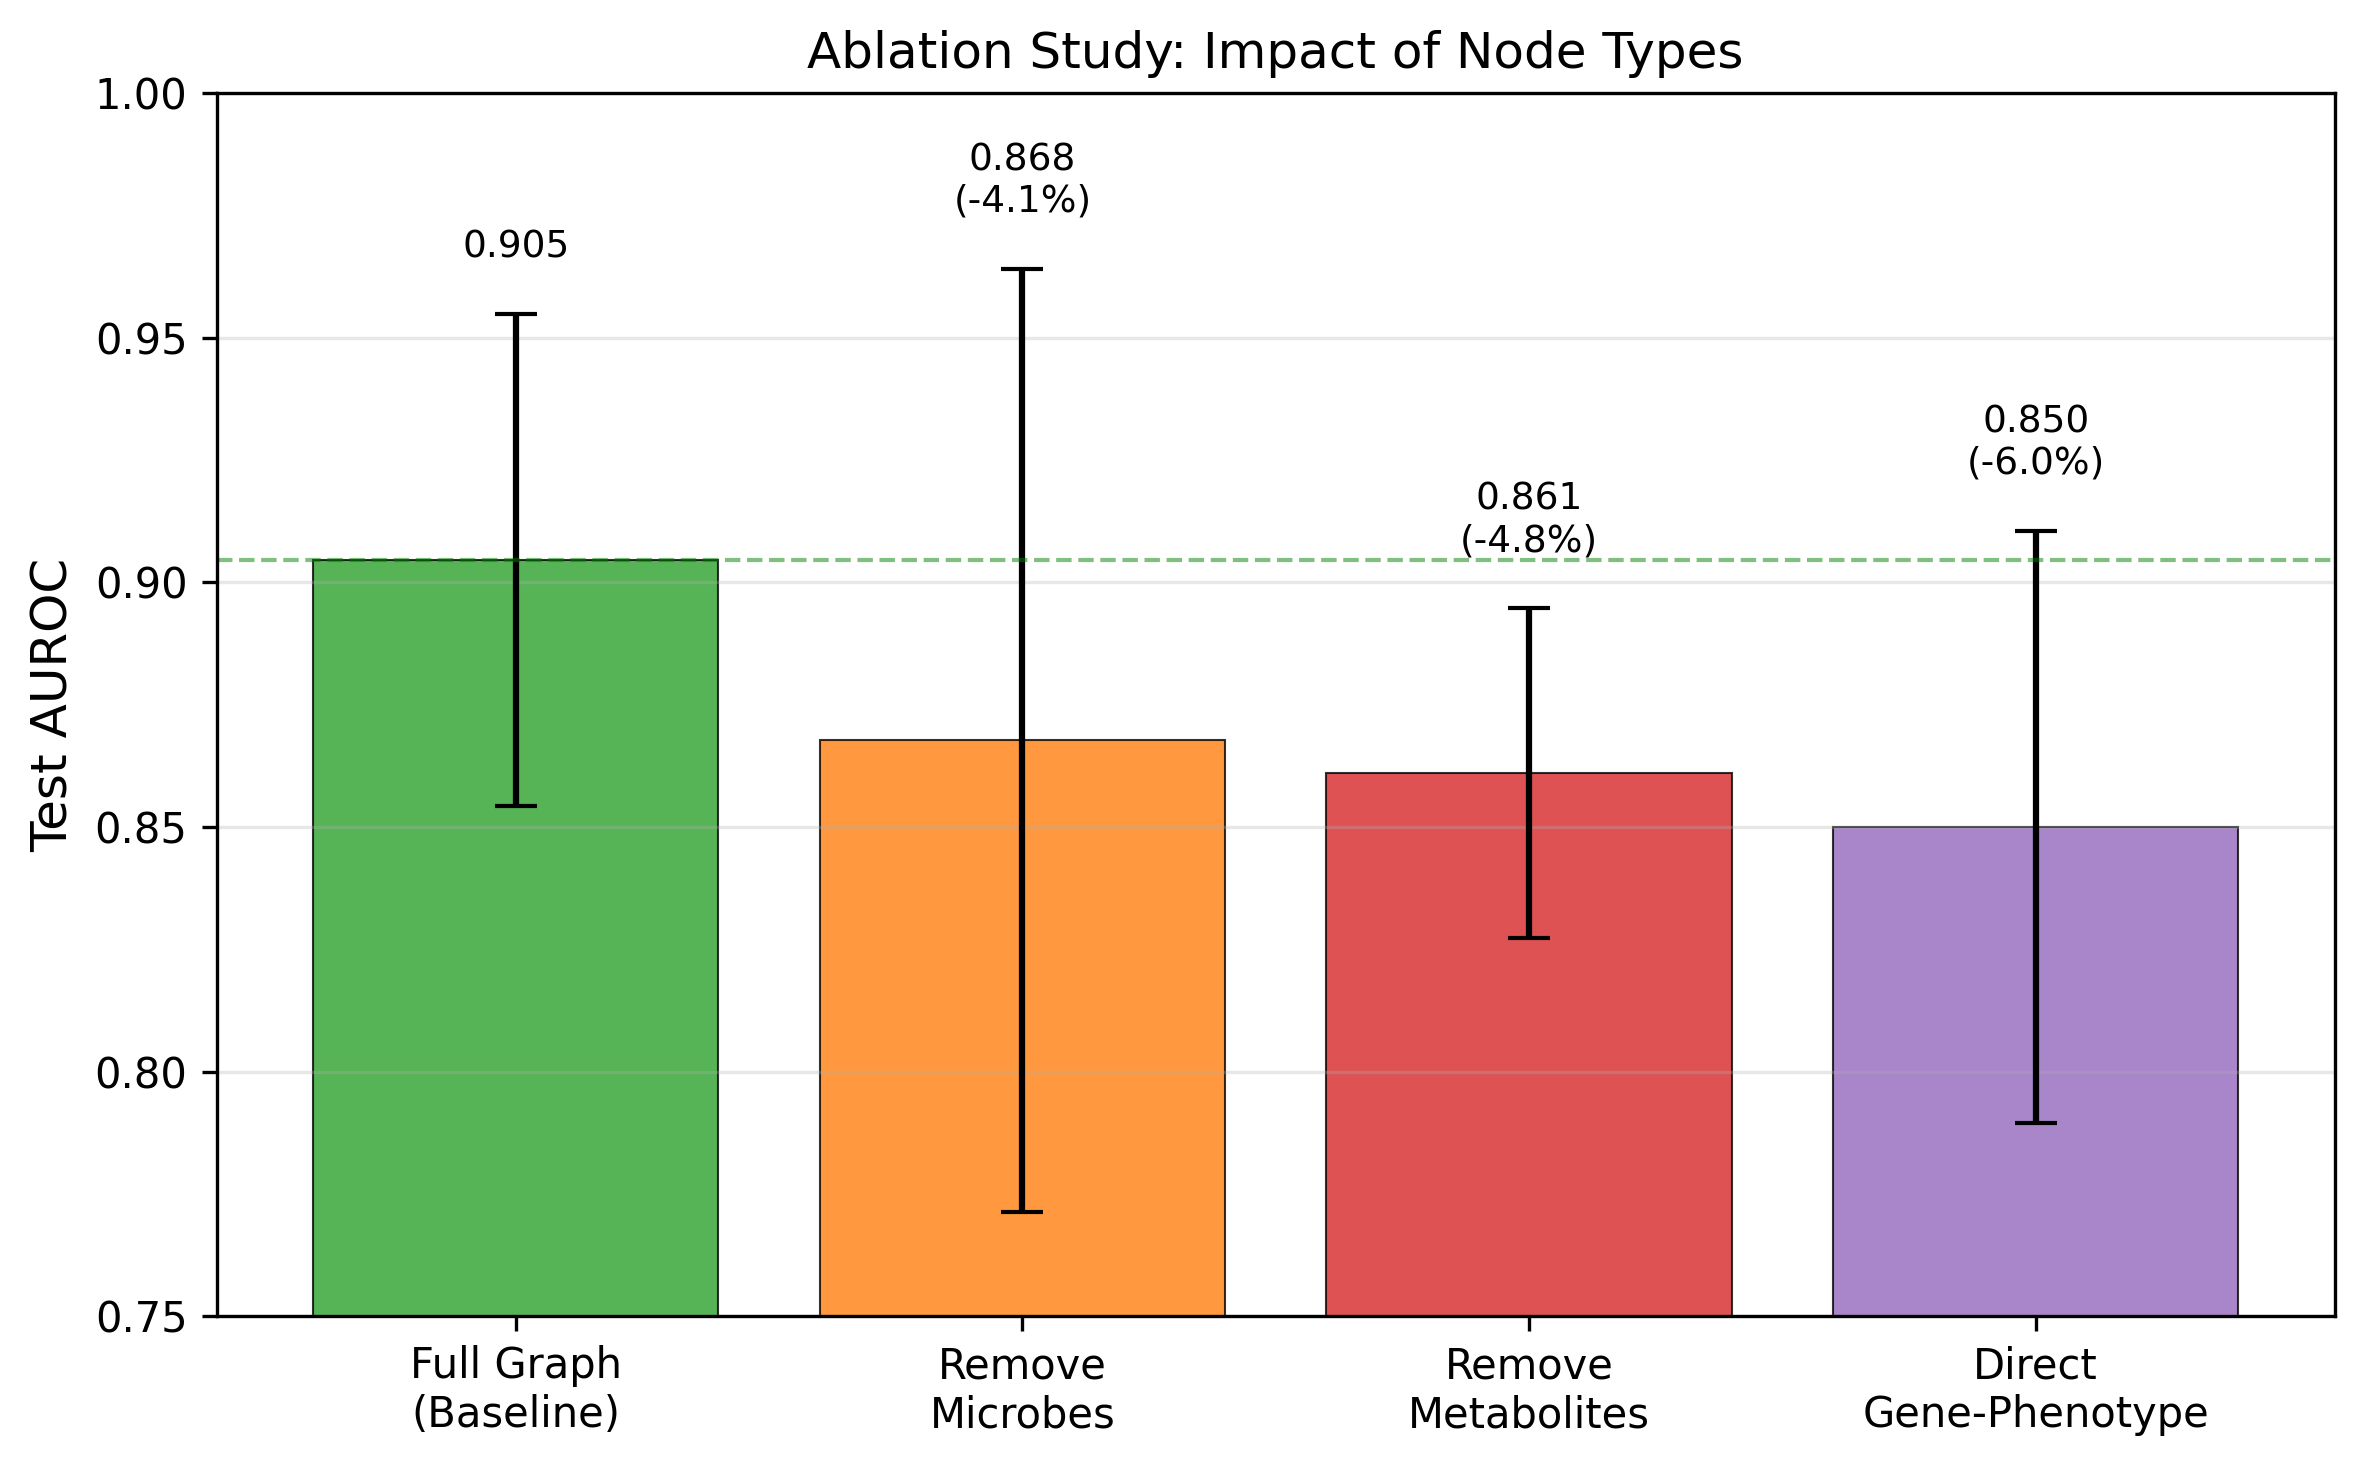
\includegraphics[width=0.85\textwidth]{../../figures/ablation_results.png}
\caption{Ablation study results showing the impact of removing node types on prediction performance. Removing metabolites causes a 4.8\% decrease in AUROC, while removing all intermediates (direct gene-phenotype only) causes a 6.0\% decrease. Error bars indicate standard deviation across 5 random seeds.}
\label{fig:ablation}
\end{figure}

Key findings from ablation studies:

\begin{enumerate}
    \item \textbf{Metabolites contribute meaningfully}: Removing metabolite nodes decreased AUROC by 4.8\%, indicating that neuroactive compounds (serotonin precursors, short-chain fatty acids) provide useful signal for predicting gene-phenotype associations.

    \item \textbf{Multi-hop reasoning helps}: The full model with both microbes and metabolites outperforms the direct gene-phenotype model by 6.0\%, suggesting that the GNN learns to propagate information through biological intermediates.

    \item \textbf{Microbe contribution is marginal}: Removing microbe nodes alone had a smaller effect (4.1\%), possibly because microbe information is already captured through their metabolite products.
\end{enumerate}

\subsection{Learned Representations}

Figure~\ref{fig:tsne} visualizes the learned node embeddings using t-SNE dimensionality reduction. The model learns representations that cluster by biological type, with genes and phenotypes positioned in proximity due to their direct associations in the training data.

\begin{figure}[h]
\centering
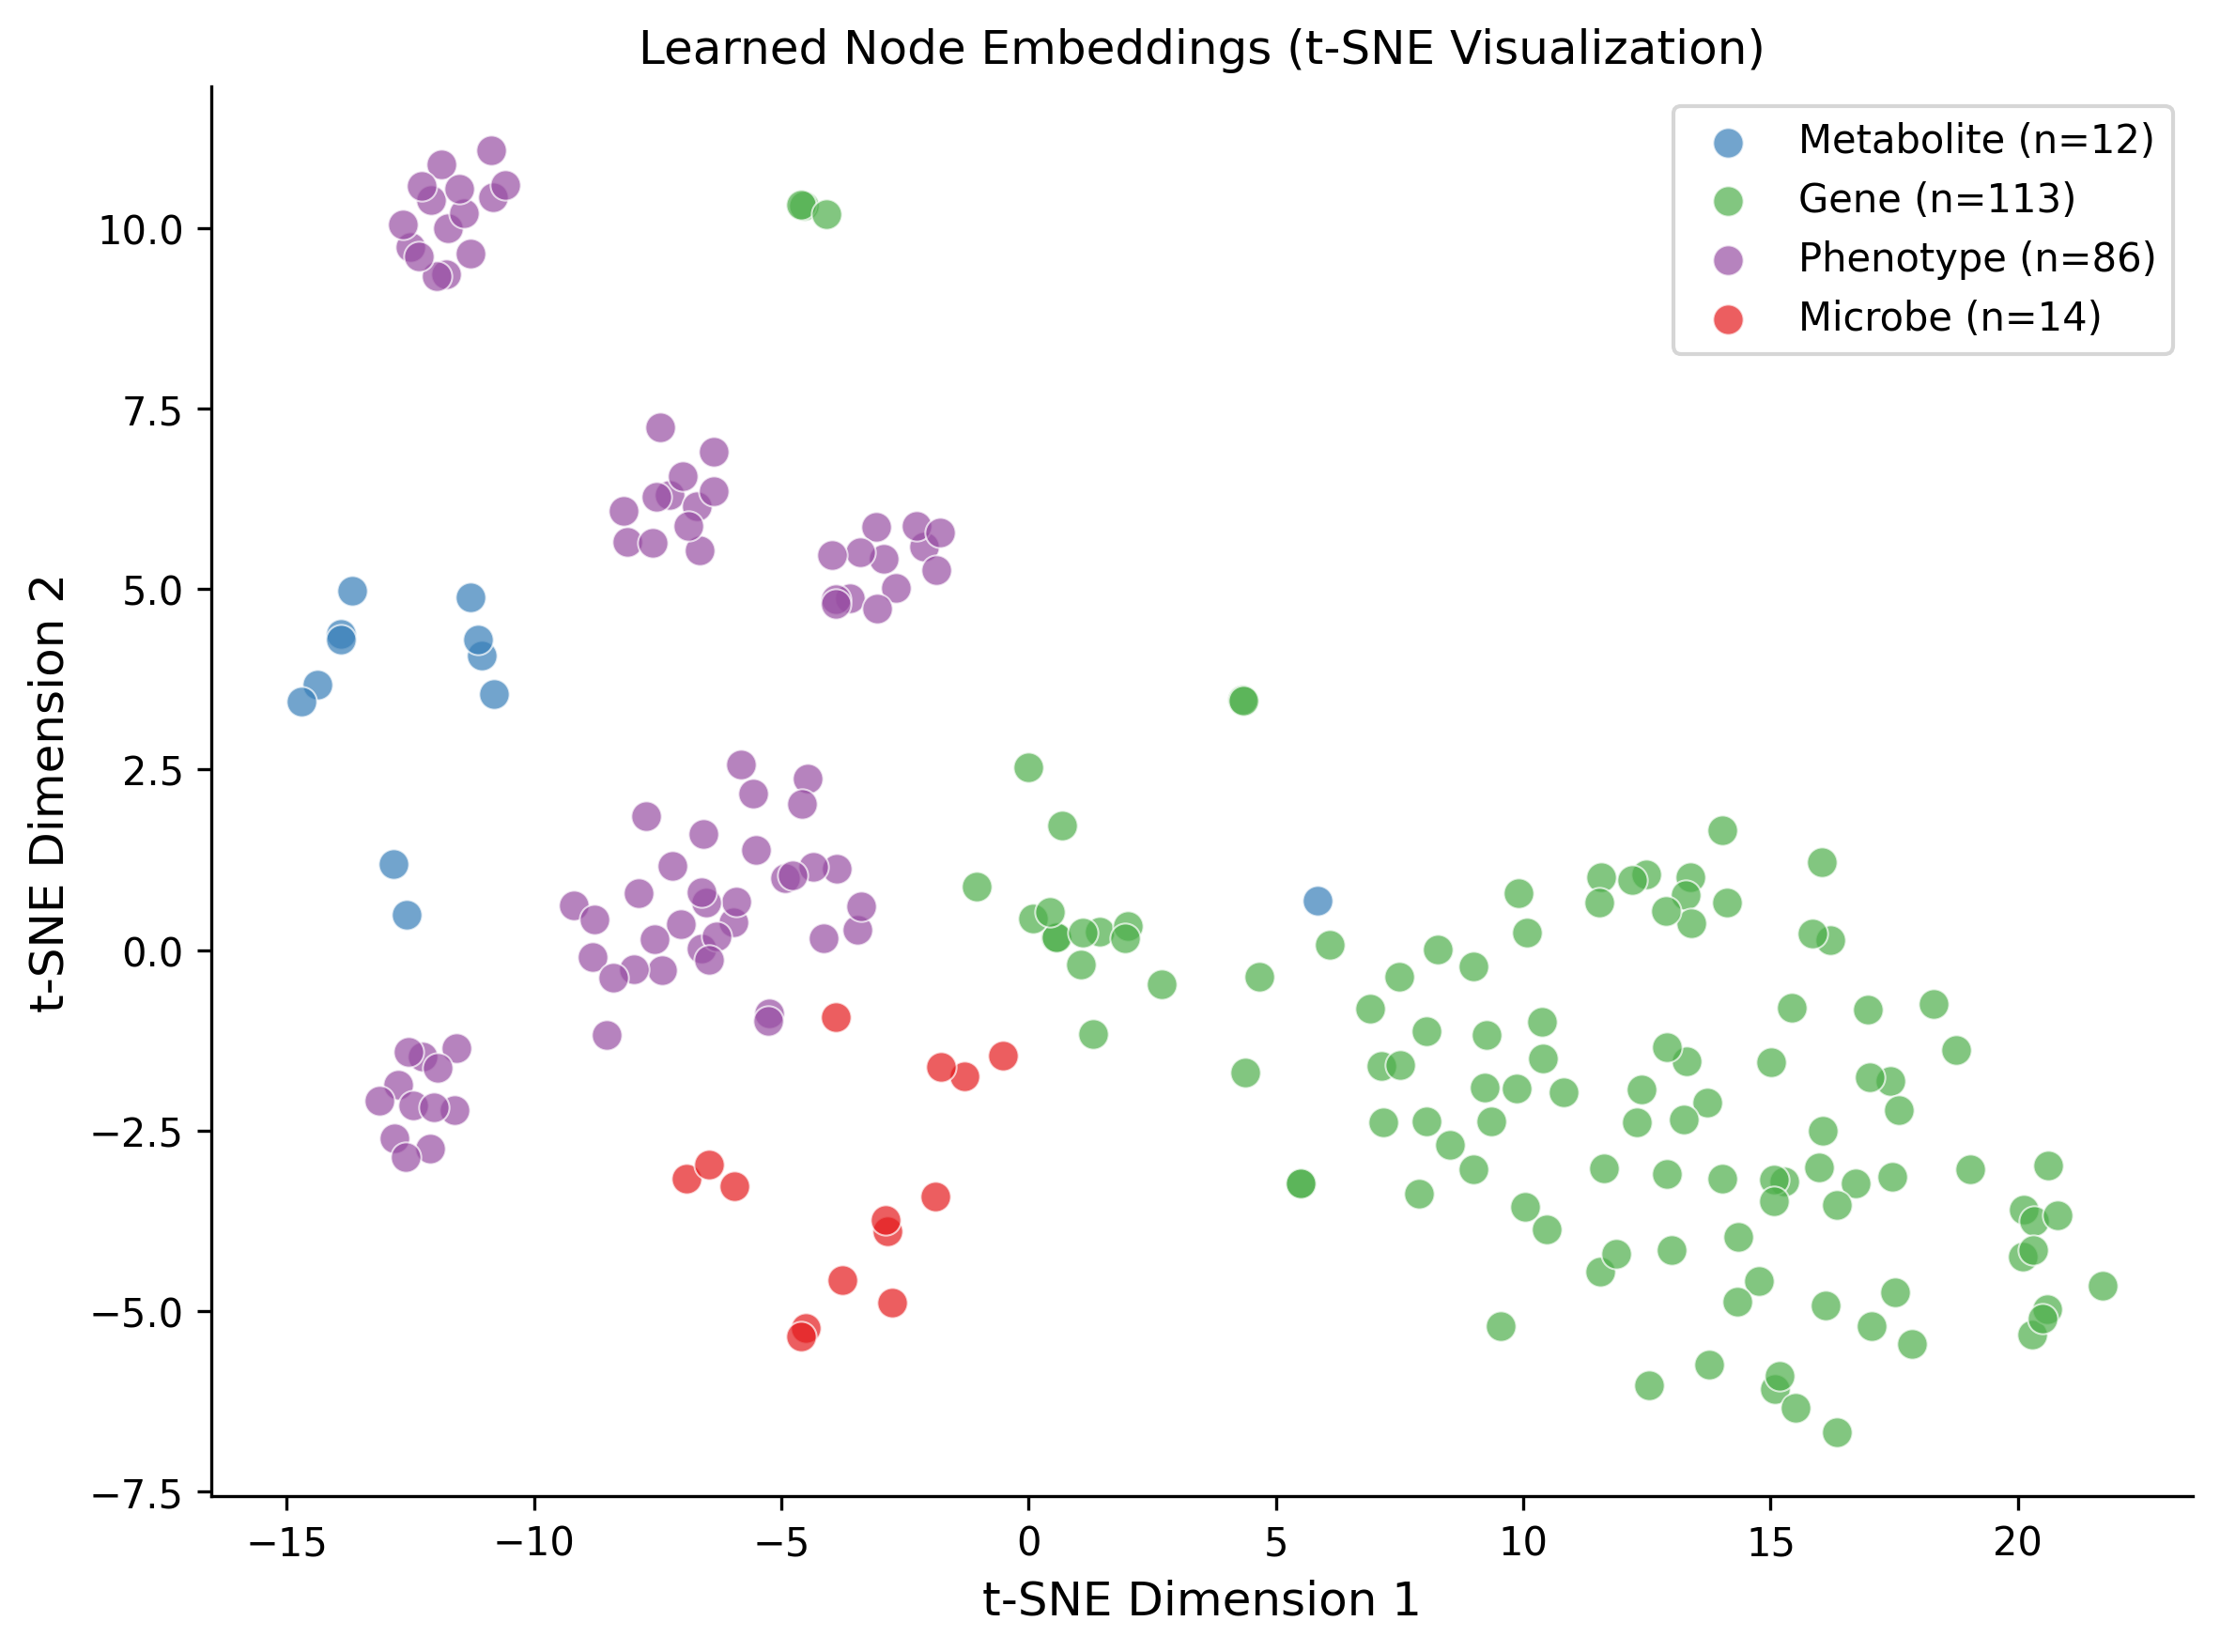
\includegraphics[width=0.75\textwidth]{../../figures/tsne_embeddings.png}
\caption{t-SNE visualization of learned node embeddings after training. Different colors represent different node types. The model learns to cluster similar entities while positioning genes and phenotypes nearby, reflecting their biological associations.}
\label{fig:tsne}
\end{figure}

% =============================================================================
\section{Discussion}

Our results demonstrate that heterogeneous graph neural networks can effectively model the complex relationships in the celiac gut-brain axis. The high prediction accuracy (AUROC = $0.905 \pm 0.050$) suggests the model captures meaningful biological signal from the curated knowledge graph.

\subsection{Biological Interpretation}

The ablation studies provide quantitative evidence for the importance of metabolic intermediates in gut-brain communication. The 4.8\% performance drop when removing metabolite nodes supports the hypothesis that neuroactive metabolites---including serotonin (95\% produced in the gut), short-chain fatty acids (affecting blood-brain barrier integrity), and tryptophan derivatives (modulating immune function)---play a role in connecting intestinal changes to neurological symptoms.

This computational finding aligns with clinical observations that:
\begin{itemize}
    \item Celiac patients show altered tryptophan metabolism \citep{russo2012tryptophan}
    \item Gluten-free diet often improves both gastrointestinal and neurological symptoms
    \item Probiotic supplementation may affect mood and cognition through metabolite production
\end{itemize}

\subsection{Limitations}

Several limitations should be acknowledged:

\begin{enumerate}
    \item \textbf{Small graph size}: With only 225 nodes and 229 edges, our knowledge graph is small compared to comprehensive biomedical KGs like PrimeKG. This limits both the complexity of learnable patterns and generalization to unseen entities.

    \item \textbf{Curation bias}: Manual edge curation may introduce systematic biases toward well-studied relationships, potentially missing novel connections.

    \item \textbf{Correlation vs. causation}: Link prediction identifies statistical associations, not causal mechanisms. Predicted links require experimental validation.

    \item \textbf{Variance across seeds}: The standard deviation of $\pm 0.050$ in AUROC indicates sensitivity to random initialization and data splitting, a known challenge for small-scale graph learning.
\end{enumerate}

\subsection{Future Directions}

Several extensions could strengthen this work:

\begin{enumerate}
    \item \textbf{Expand the knowledge graph}: Incorporate additional data sources (STRING protein interactions, DrugBank, metabolomic datasets) to increase coverage

    \item \textbf{Add expression data}: Integrate gene expression profiles from celiac patient biopsies to weight edges by disease relevance

    \item \textbf{Multi-task prediction}: Extend to predict microbe-phenotype and metabolite-phenotype links for a more complete picture of gut-brain interactions

    \item \textbf{Experimental validation}: Collaborate with wet-lab researchers to test top-ranked predictions in cell culture or animal models
\end{enumerate}

% =============================================================================
\section{Conclusion}

We developed a graph-based machine learning approach to model the celiac gut-brain axis using heterogeneous graph neural networks. Our curated knowledge graph integrates microbiome, metabolite, gene, and phenotype data into a unified representation, achieving AUROC of $0.905 \pm 0.050$ on gene-phenotype link prediction across five random seeds.

Ablation studies demonstrate that metabolic intermediates contribute meaningfully to prediction accuracy, providing computational support for the role of neuroactive metabolites in gut-brain communication. The 6.0\% performance improvement when including microbe and metabolite nodes suggests that multi-hop message passing captures biologically relevant information flow from gut bacteria to neurological outcomes.

This computational framework generates testable hypotheses for understanding gut-brain communication in celiac disease and provides a template for applying graph neural networks to other complex multi-system diseases.

% =============================================================================
\section*{Acknowledgments}
We thank [mentors/advisors] for guidance and feedback on this project.

\section*{Data and Code Availability}
All code and data are available at: \url{https://github.com/[repository]}

\section*{Author Contributions}
[Author] designed the study, curated the knowledge graph, implemented the models, ran experiments, and wrote the manuscript.

% =============================================================================
\bibliographystyle{plainnat}
\bibliography{references}

\begin{thebibliography}{99}

\bibitem{lebwohl2018celiac}
Lebwohl, B., Sanders, D. S., \& Green, P. H. (2018).
Coeliac disease.
\textit{The Lancet}, 391(10115), 70-81.

\bibitem{caio2019celiac}
Caio, G., Volta, U., Sapone, A., et al. (2019).
Celiac disease: a comprehensive current review.
\textit{BMC Medicine}, 17(1), 142.

\bibitem{hadjivassiliou2008autoantibodies}
Hadjivassiliou, M., Aeschlimann, P., Sanders, D. S., et al. (2008).
Autoantibodies in gluten ataxia recognize a novel neuronal transglutaminase.
\textit{Annals of Neurology}, 64(3), 332-343.

\bibitem{dinan2017gutbrain}
Dinan, T. G., \& Cryan, J. F. (2017).
Gut-brain axis in 2016: Brain-gut-microbiota axis - mood, metabolism and behaviour.
\textit{Nature Reviews Gastroenterology \& Hepatology}, 14(2), 69-70.

\bibitem{arcila2022microbiome}
Arcila-Galvis, J. E., et al. (2022).
Systematic review of the gut microbiome in celiac disease.
\textit{Gut Microbes}, 14(1), 2087291.

\bibitem{zhang2022graph}
Zhang, Z., et al. (2022).
Graph neural networks and their applications in drug discovery.
\textit{Expert Opinion on Drug Discovery}, 17(1), 1-13.

\bibitem{fey2019pyg}
Fey, M., \& Lenssen, J. E. (2019).
Fast graph representation learning with PyTorch Geometric.
\textit{ICLR Workshop on Representation Learning on Graphs and Manifolds}.

\bibitem{hamilton2017graphsage}
Hamilton, W., Ying, Z., \& Leskovec, J. (2017).
Inductive representation learning on large graphs.
\textit{Advances in Neural Information Processing Systems}, 30.

\bibitem{russo2012tryptophan}
Russo, P., Ferranti, P., Gianfrani, C., et al. (2012).
Altered tryptophan metabolism in celiac disease.
\textit{Neuroimmunomodulation}, 19(4), 239-248.

\end{thebibliography}

\end{document}
